\section{TỔNG QUAN HỆ THỐNG}\label{sec:chuong1}

Hệ thống gây quỹ cộng đồng Góp Mầm được thiết kế để quản lý toàn bộ quy trình từ đăng ký tài khoản, tạo và kiểm duyệt chiến dịch, ủng hộ trực tuyến kèm mức quà, cập nhật tiến độ giải ngân có chứng từ, hoàn tiền, đến tương tác cộng đồng, kiểm duyệt vi phạm, phát hiện gian lận bằng AI, thông báo, xác minh tổ chức thụ hưởng và xác minh bổ sung bằng mã OTP cho thao tác nhạy cảm. Hệ thống gồm 24 thực thể với 37 mối quan hệ có khóa ngoại và 5 tham chiếu logic.

Hệ quản trị cơ sở dữ liệu: MySQL 8, engine InnoDB. Schema chỉ thay đổi qua migration TypeORM có thứ tự và có rollback (khớp tới migration 1790000000012).

Các thực thể được chia thành sáu nhóm nghiệp vụ như Bảng~\ref{tab:nhom_thuc_the}.

\begin{table}[htbp]
    \centering
    \small
    \caption{Các nhóm thực thể}
    \label{tab:nhom_thuc_the}
    \begin{tabularx}{\textwidth}{|P{3.6cm}|X|}
        \hline
        \textbf{Nhóm} & \textbf{Thực thể} \\
        \hline
        Tài khoản & USERS, EMAIL\_\allowbreak{}VERIFICATION\_\allowbreak{}TOKENS, PASSWORD\_\allowbreak{}RESET\_\allowbreak{}TOKENS, REVOKED\_\allowbreak{}TOKENS, STEP\_\allowbreak{}UP\_\allowbreak{}CODES \\
        \hline
        Chiến dịch và tiến độ & CAMPAIGNS, ORGANIZATIONS, CATEGORIES, CAMPAIGN\_\allowbreak{}VIEW\_\allowbreak{}DAILY, MILESTONES, MILESTONE\_\allowbreak{}UPDATES, MILESTONE\_\allowbreak{}UPDATE\_\allowbreak{}ATTACHMENTS, MILESTONE\_\allowbreak{}REVISIONS, REWARD\_\allowbreak{}TIERS, MEDIA\_\allowbreak{}FILES \\
        \hline
        Giao dịch & DONATIONS, REFUND\_\allowbreak{}REQUESTS \\
        \hline
        Cộng đồng & CAMPAIGN\_\allowbreak{}COMMENTS, CAMPAIGN\_\allowbreak{}FOLLOWS \\
        \hline
        Kiểm duyệt và rủi ro & REPORTS, RISK\_\allowbreak{}ALERTS \\
        \hline
        AI và hệ thống & BEHAVIOR\_\allowbreak{}EVENTS, NOTIFICATIONS, AUDIT\_\allowbreak{}LOGS \\
        \hline
    \end{tabularx}
\end{table}

\subsection{Sơ đồ ERD}

Sơ đồ dưới đây thể hiện các thực thể và quan hệ có khóa ngoại. Hình ERD vật lý đầy đủ cột được vẽ tự động (Graphviz) từ file DBML docs/database/schema.dbml.

\begin{figure}[htbp]
    \centering
    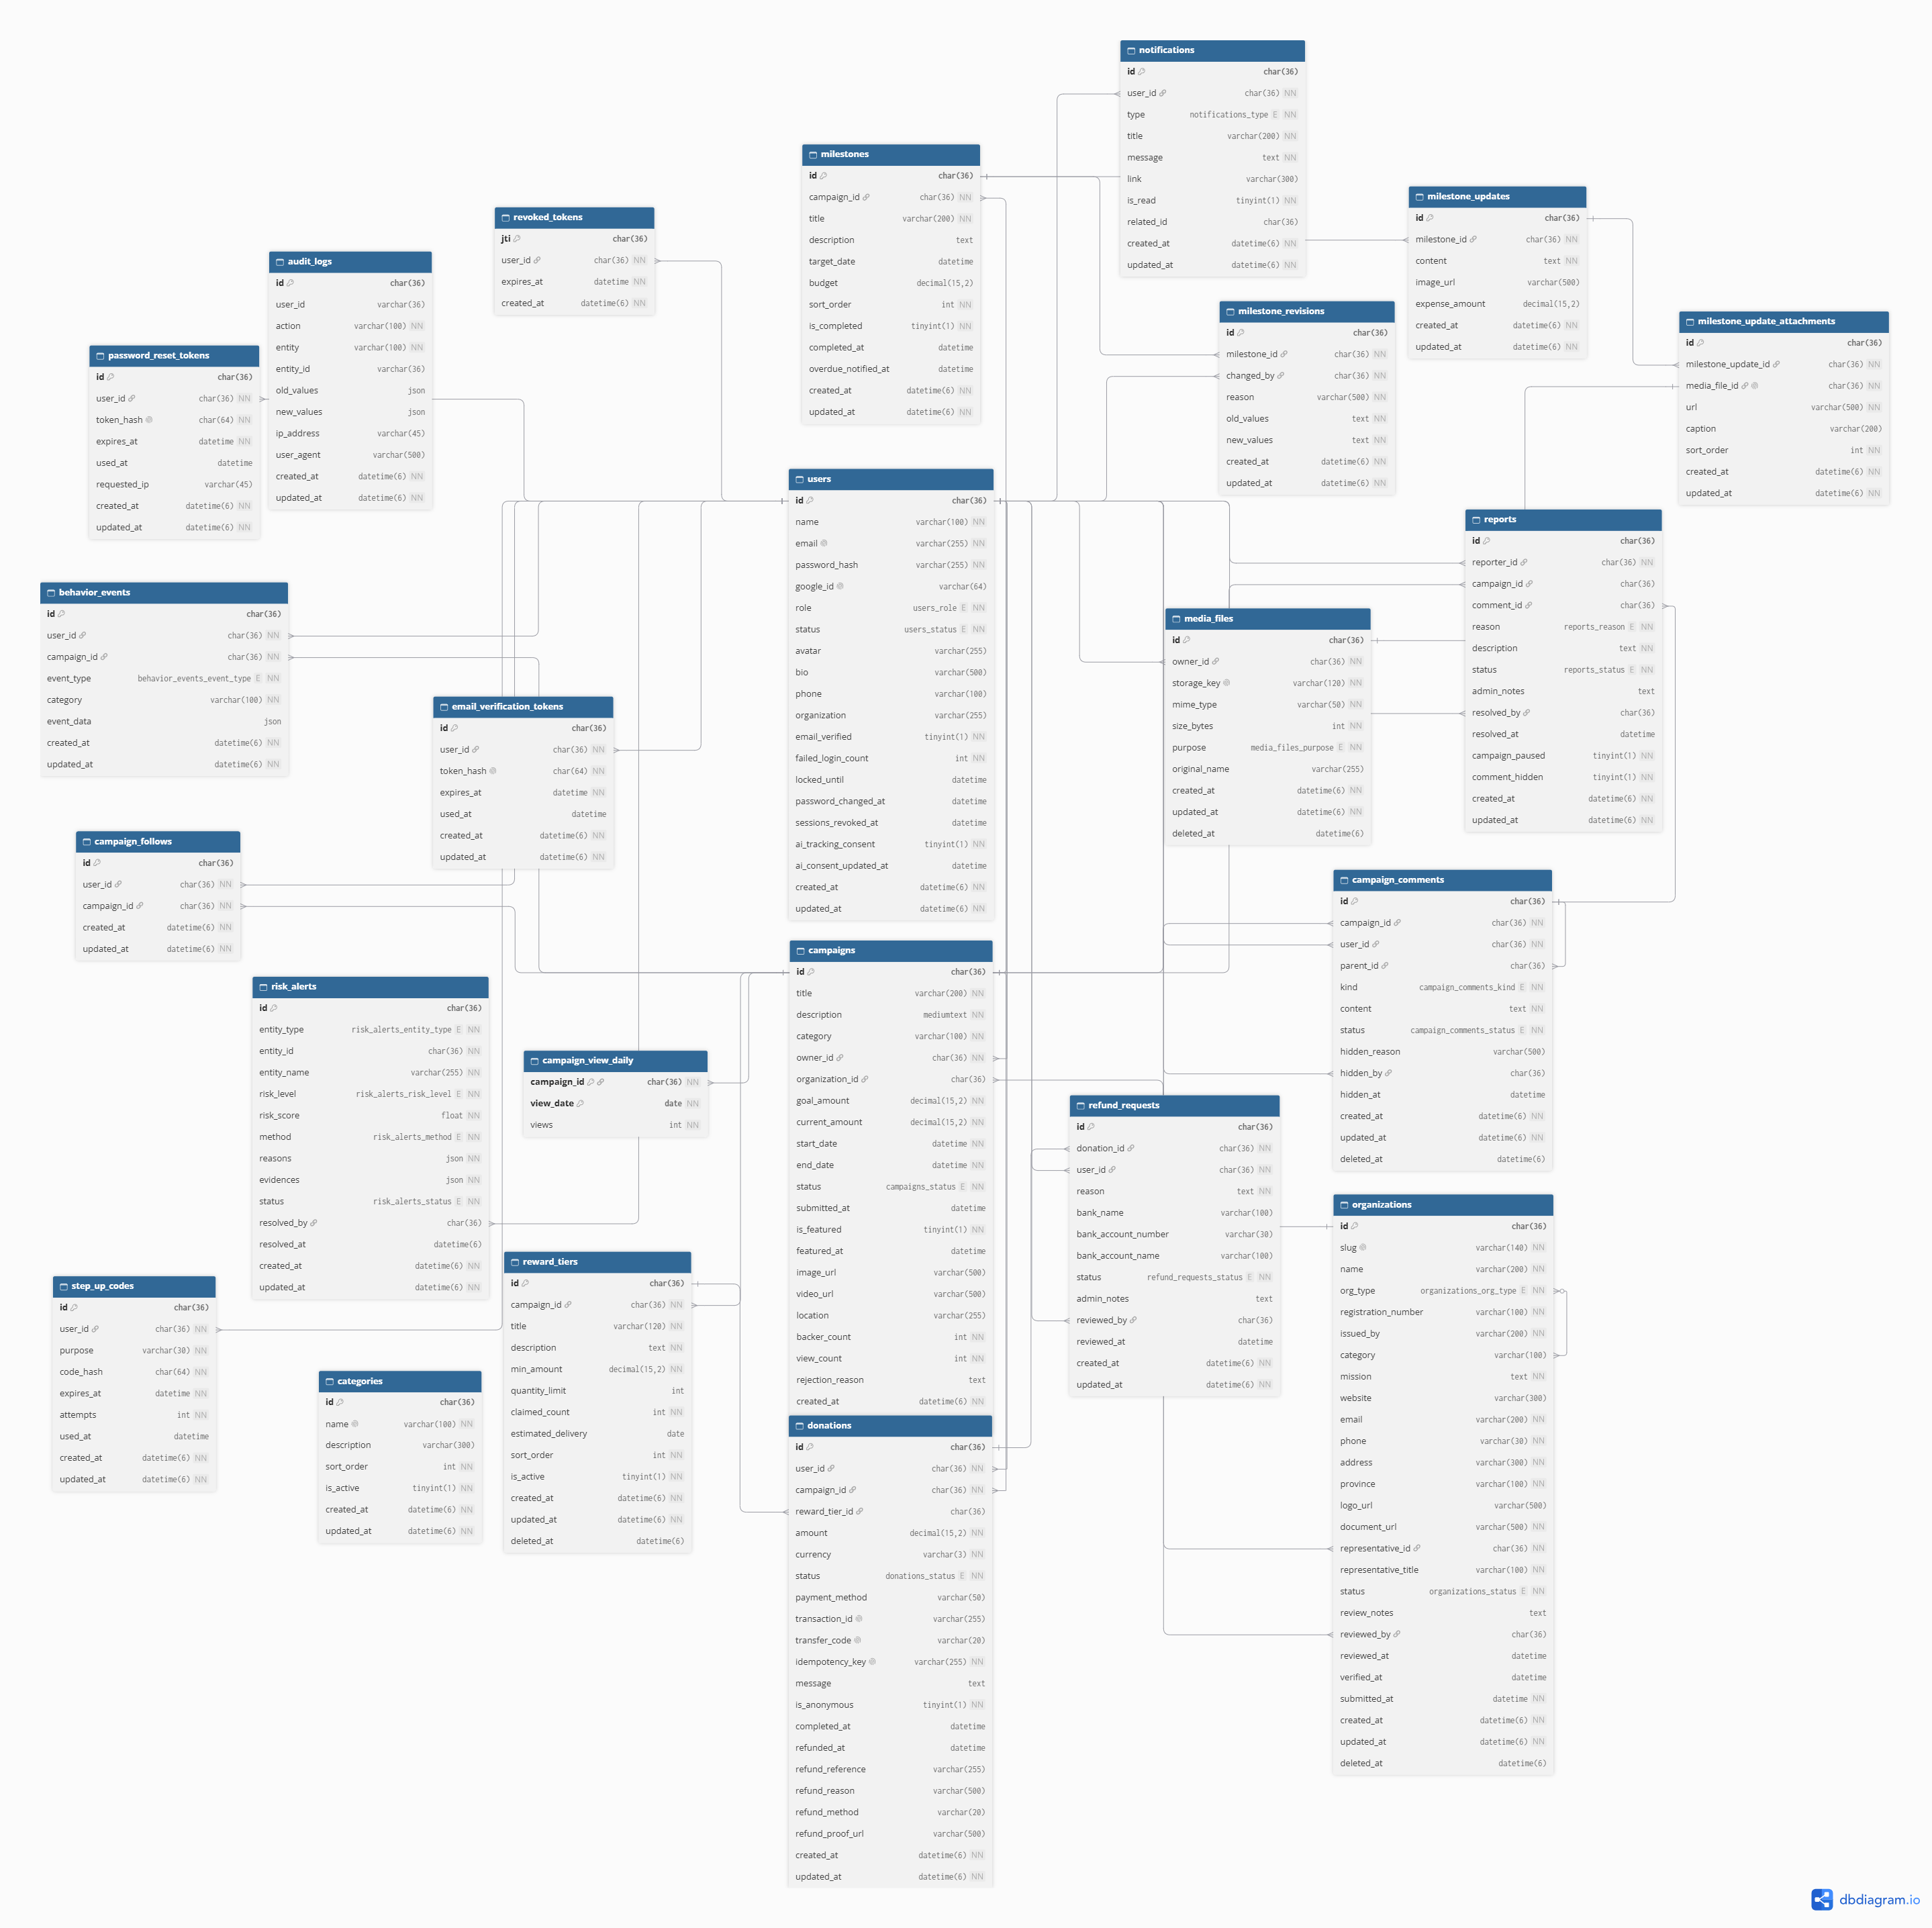
\includegraphics[width=\textwidth,height=0.72\textheight,keepaspectratio]{image/ERD_GopMam.png}
    \caption{Sơ đồ ERD vật lý hệ thống Góp Mầm (24 bảng)}
    \label{fig:erd_vat_ly}
\end{figure}

\subsection{Mô hình quan hệ}

Mô hình quan hệ (ký hiệu Chen) vẽ các thực thể bằng hình chữ nhật và quan hệ bằng hình thoi, tên quan hệ lấy theo các mục ở Chương 3. Sơ đồ lõi của hệ thống được vẽ ở cuối chương này.

\begin{figure}[htbp]
    \centering
    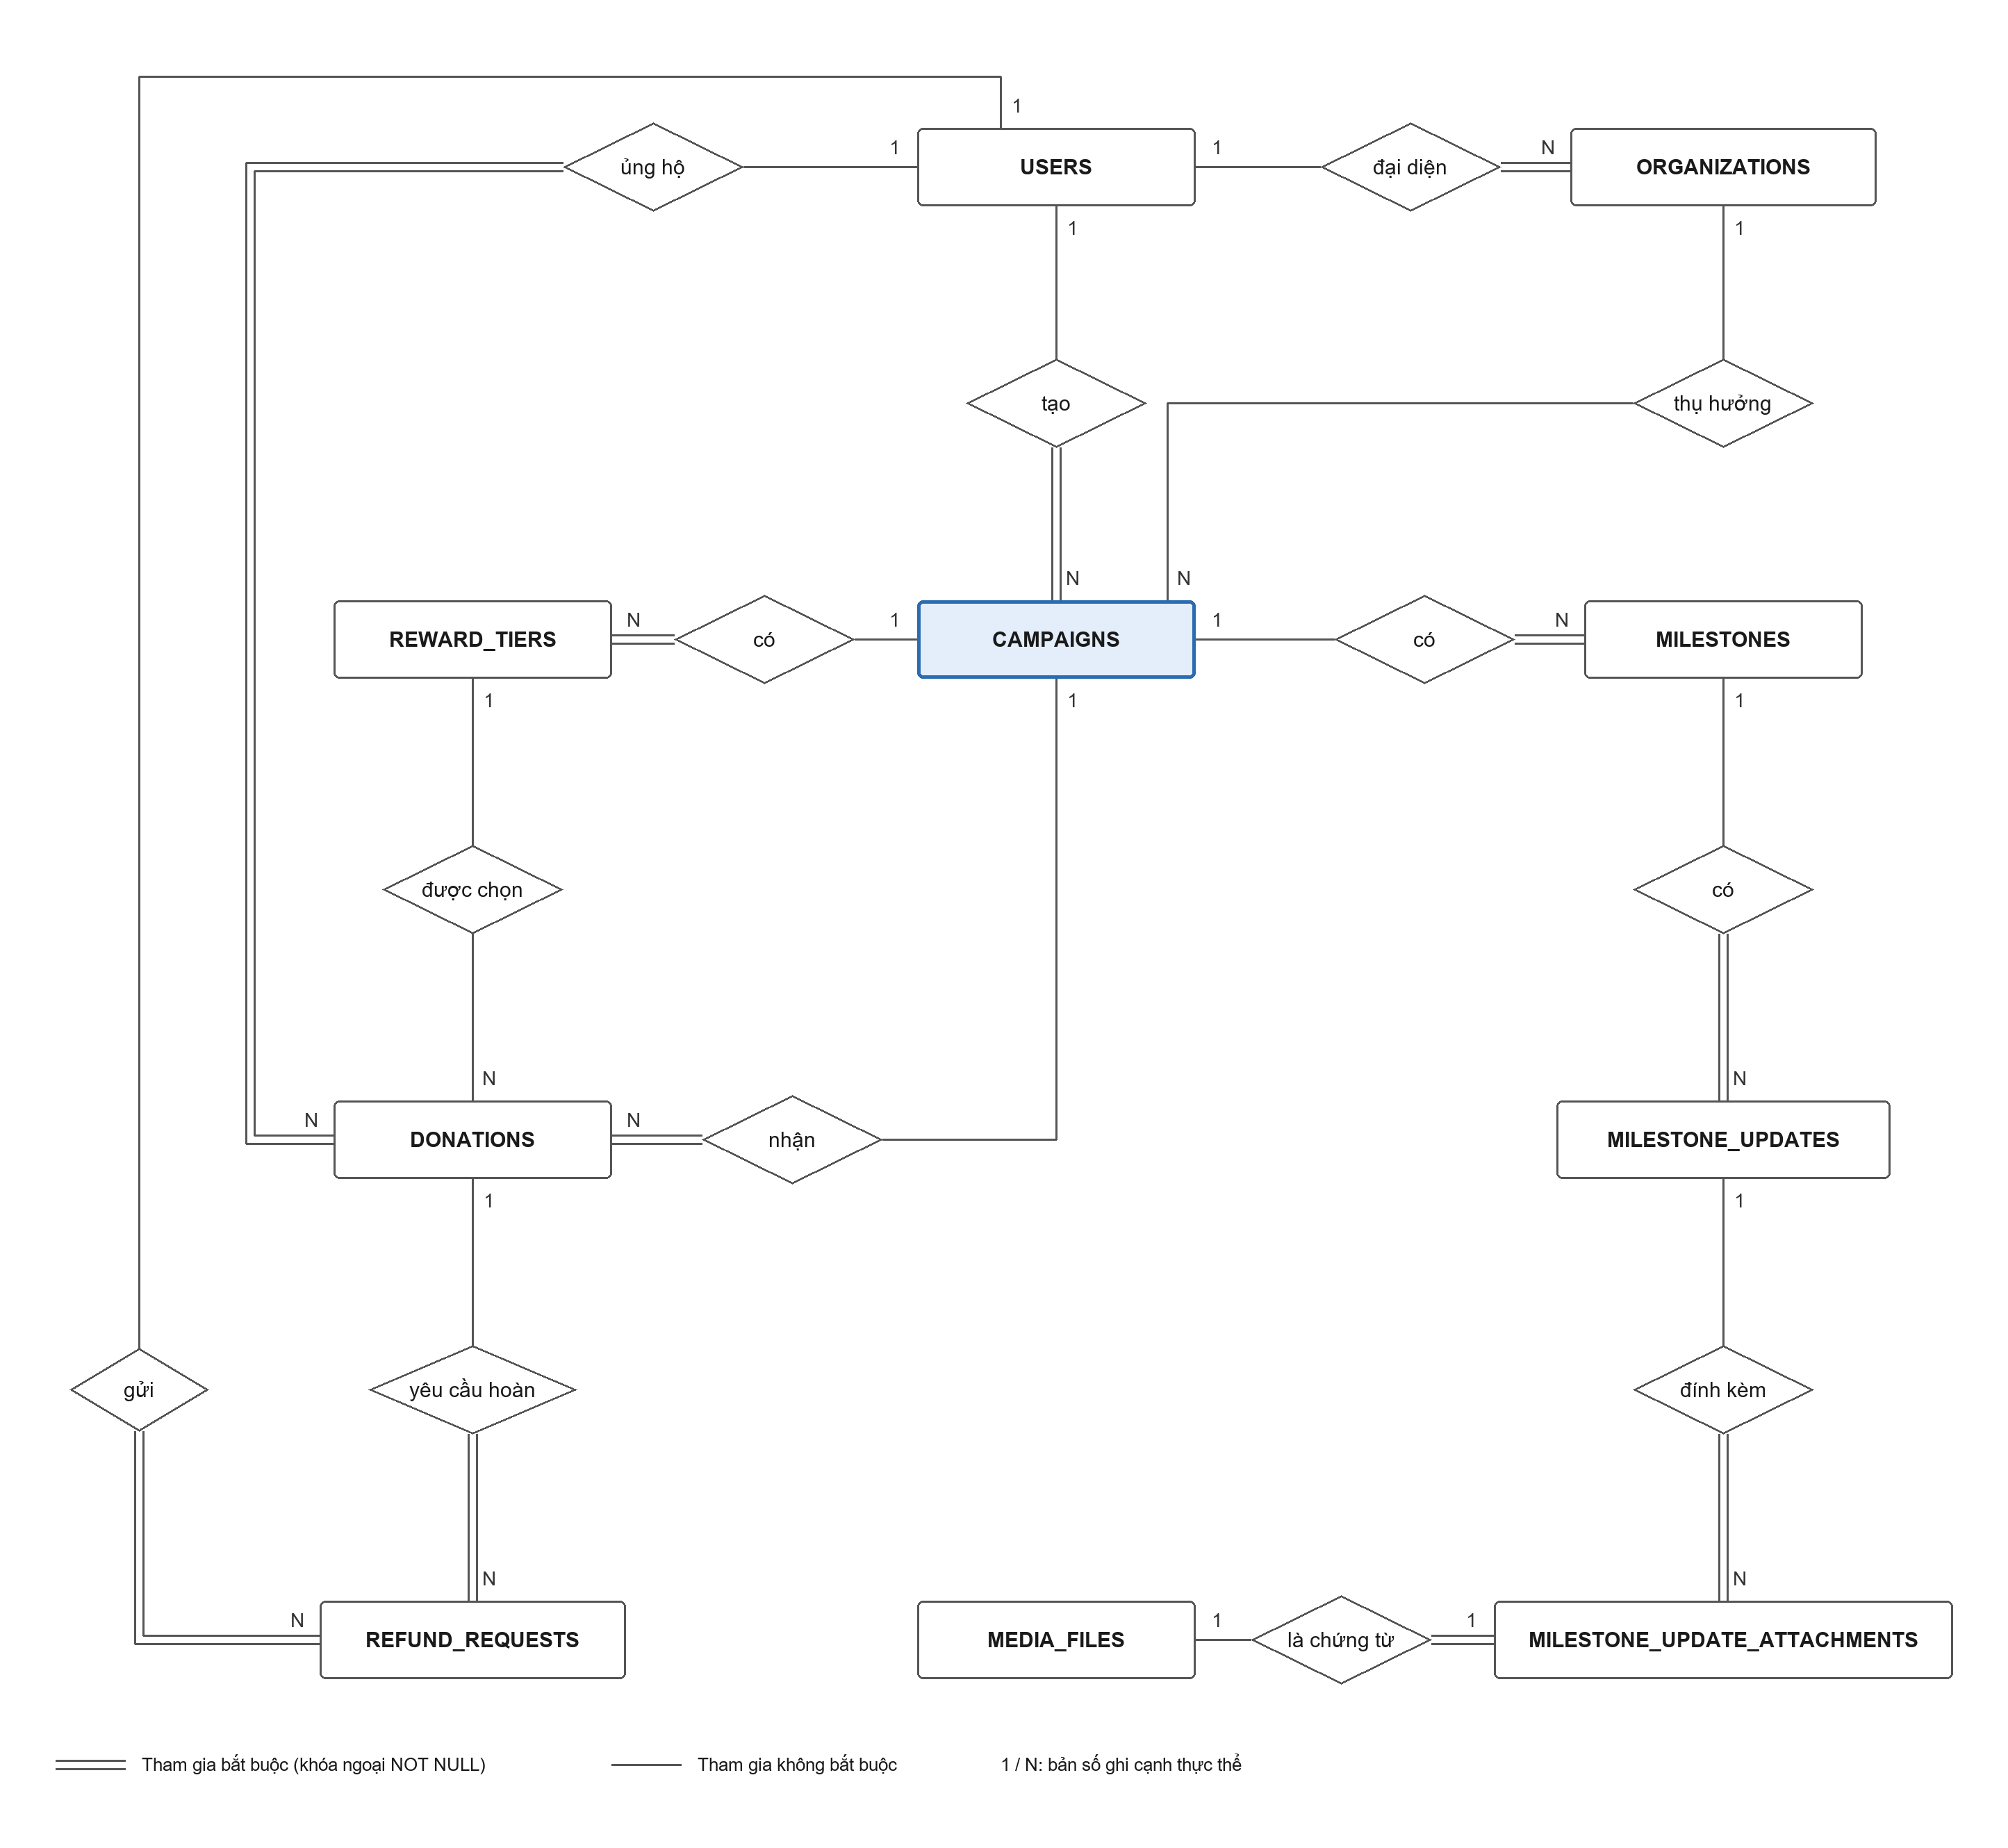
\includegraphics[width=\textwidth,height=0.72\textheight,keepaspectratio]{image/MoHinhQuanHe_GopMam.png}
    \caption{Mô hình quan hệ lõi (ký hiệu Chen)}
    \label{fig:mo_hinh_quan_he}
\end{figure}

Hình gồm các thực thể lõi của luồng gây quỹ (kể cả tổ chức thụ hưởng), ủng hộ, hoàn tiền và giải ngân; nét đôi là phía tham gia bắt buộc (khóa ngoại NOT NULL). Đủ 24 thực thể và 37 quan hệ được đặc tả ở Chương 2 và Chương 3.
